\chapter{System Characteristics from a Functional Point of View}\label{cap:functions}

After detailing the requirements, the chosen architecture for the system, the technologies used in the project, and the detailing of the implementation of each system component, this chapter is focused on the functionalities that make up the application. The project encompasses several components, including a frontend layer, a backend layer, a data receiving module, a data processing module, and the database. Therefore, this chapter aims to detail the operation of each system functionality, providing a comprehensive view of how each component interacts and contributes to the operation of the system as a whole.

Each section of this chapter will be dedicated to a specific functionality, examining its role and operation in depth, as well as the interaction between different system components for its realization.


\section[Real-time Monitoring]{Real-time Monitoring}\label{sec:realtimeMonitoring}

\begin{figure}[htbp]
	\centering
	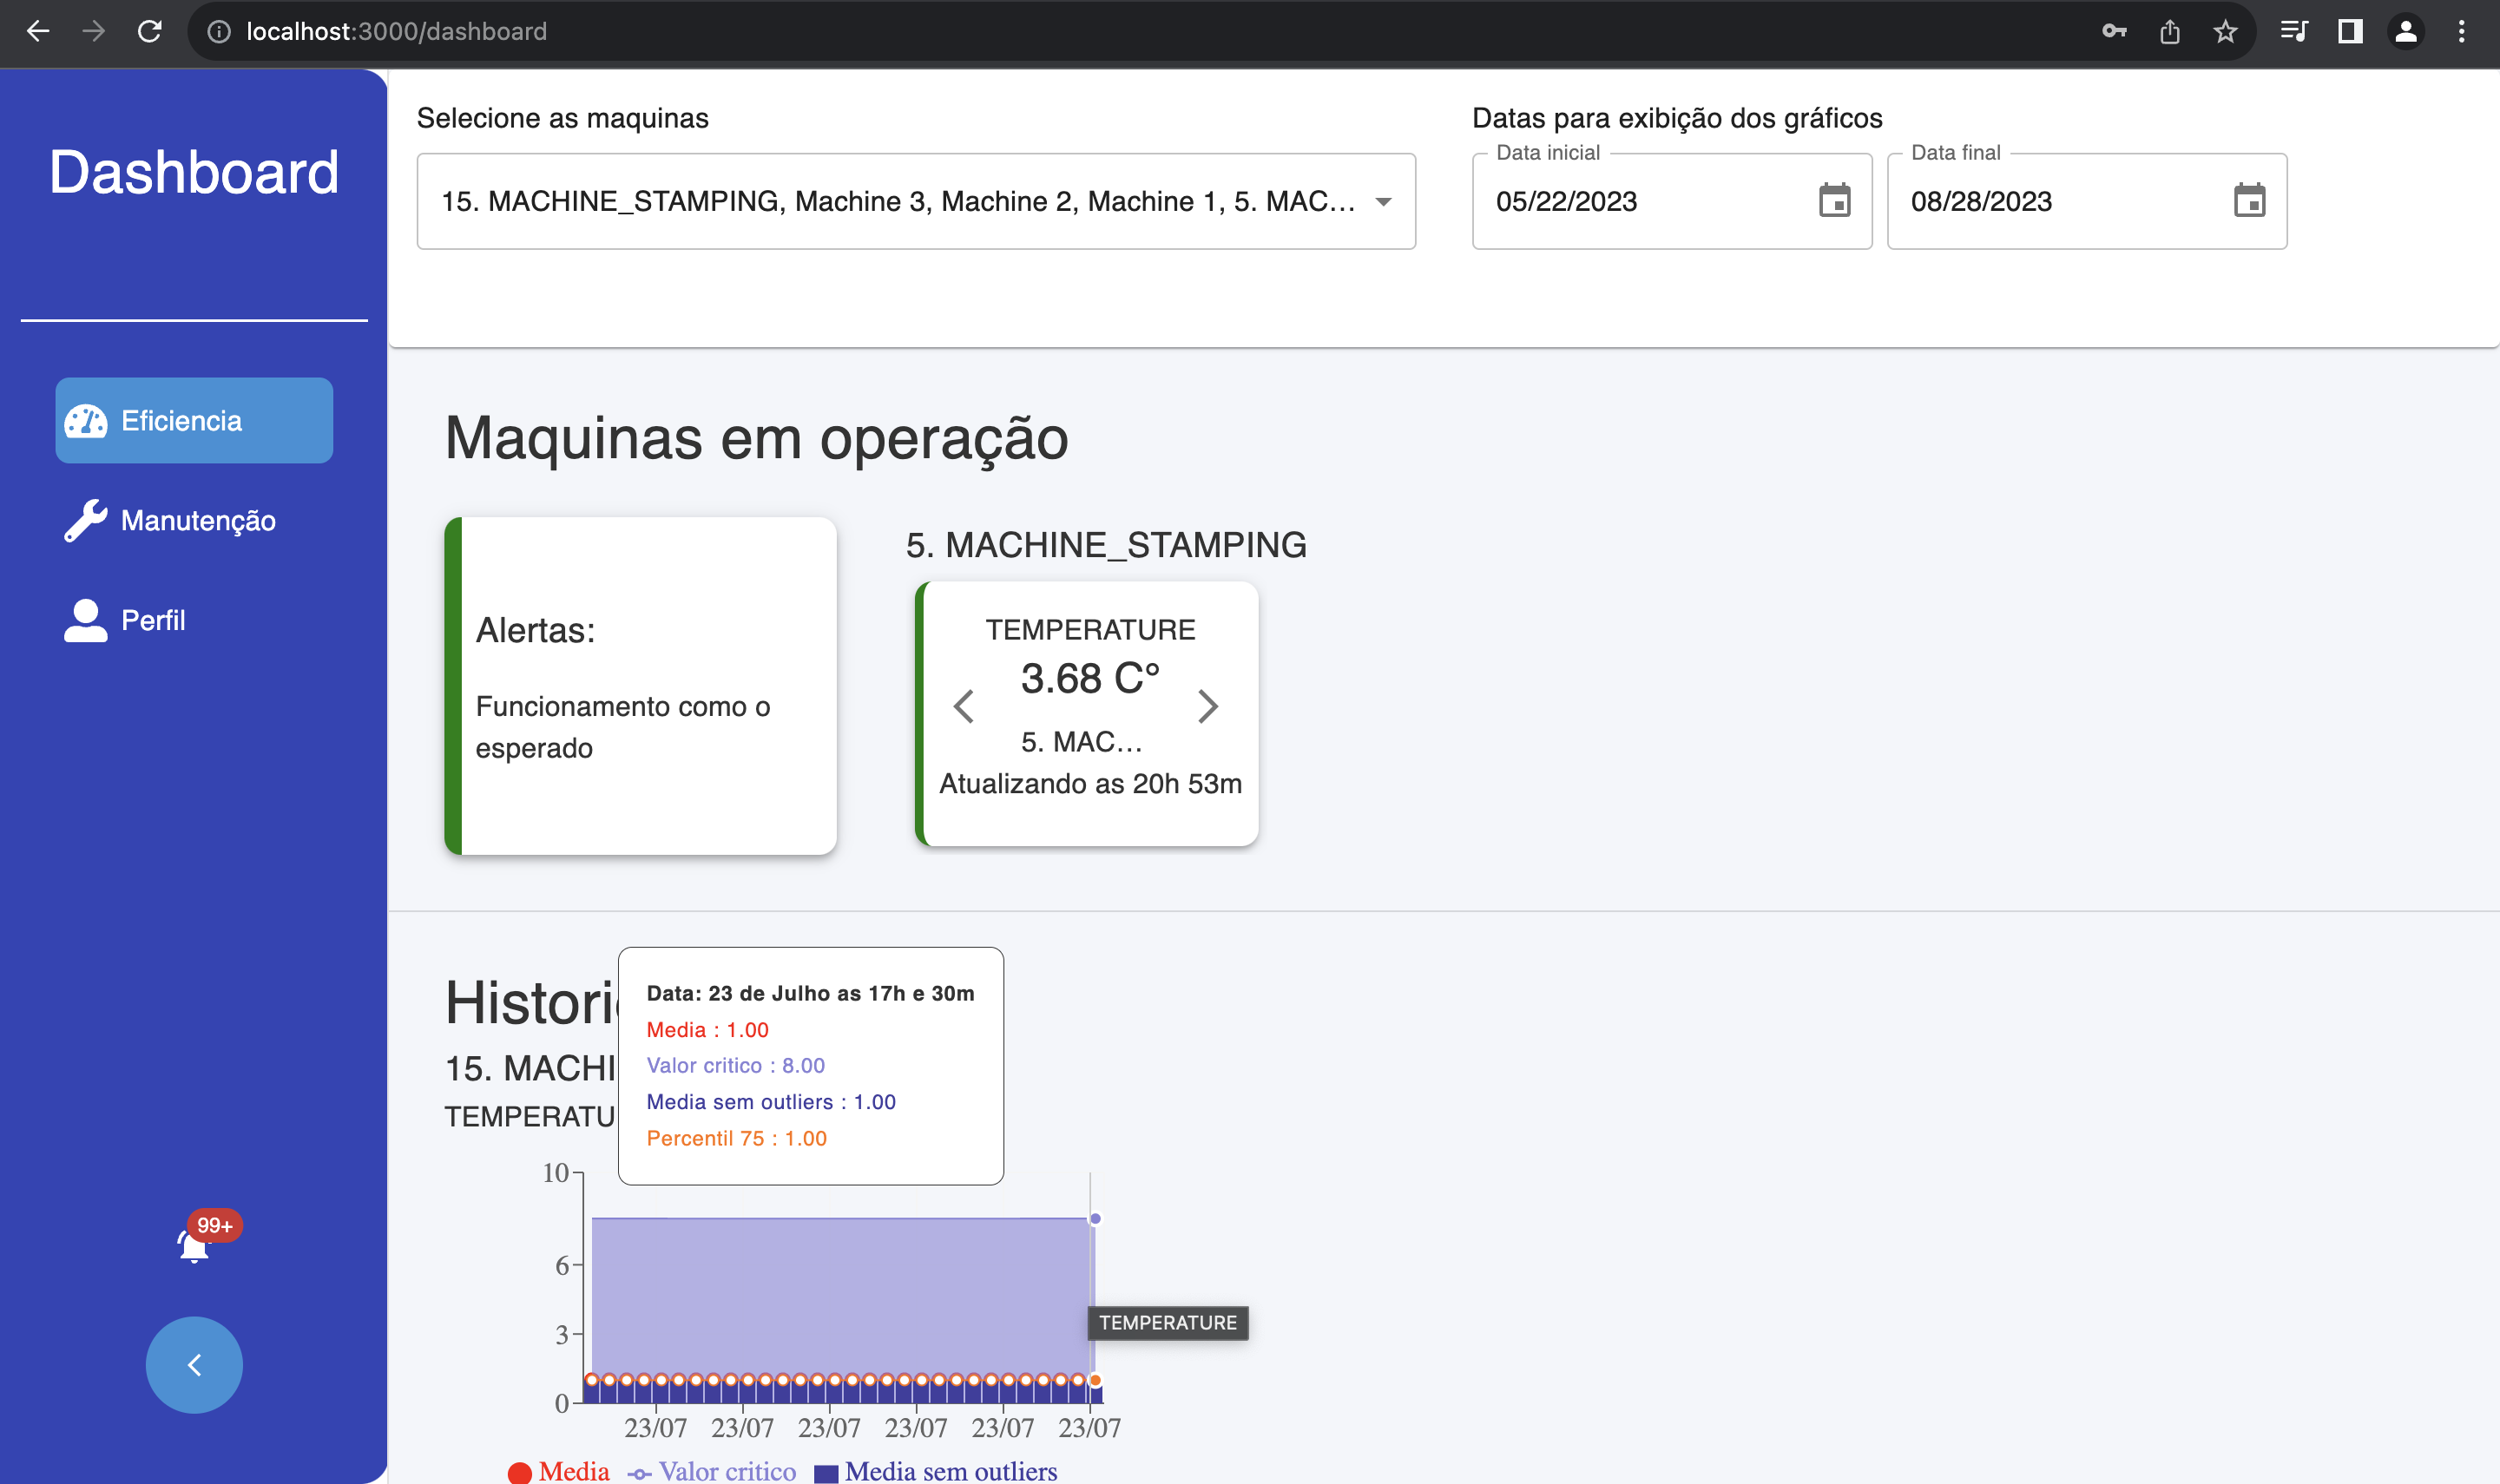
\includegraphics[scale=0.22]{images/dashboard.png}
	\caption{Dashboard with real time and graph data.}
	\label{fig:dashboradPage}
\end{figure}

On the user interface dashboard, individual cards corresponding to each monitored machine are presented. In figure \ref{fig:dashboradPage}, this page can be seen with a card for the machine \texttt{5. MACHINE\_STAMPING}. On each card, sensor information is displayed with the possibility of navigating between them with a directional arrow. The card can be seen in figure \ref{fig:cardData}.

\begin{figure}[htbp]
	\centering
	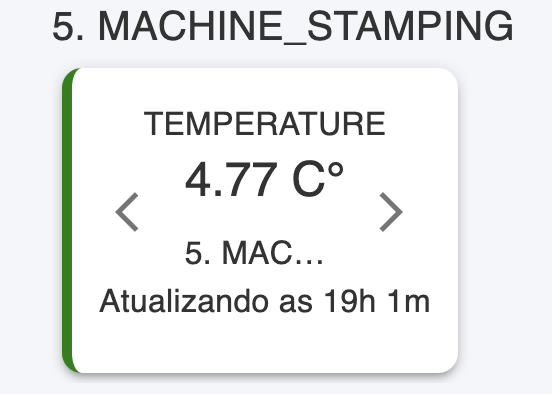
\includegraphics[scale=0.45]{images/machineCard.png}
	\caption{Card with machine data.}
	\label{fig:cardData}
\end{figure}

The acquisition of this real-time data is carried out through a continuous data stream. The frontend of the application makes a request to the endpoint \texttt{iot/realtime}, which returns this real-time data stream. The provision of this information occurs as explained in \ref{subsec:api_access}.

In the backend layer, the data stream is constantly fed by the \texttt{SensorValue} class, which in turn, is updated by the data receiving module. Upon receiving new sensor readings, the module performs appropriate validations before updating the values in the \texttt{SensorValue} class, as explained in \ref{sec:Implementation of the data receiving module}. Once updated, the \gls{API} accesses these new values and inserts them into the data stream transmitted to the connected user.


\section[Alerts and notifications]{Alerts and notifications}\label{sec:alertsAndNotifications}

The main objective of this feature is to monitor the performance of the machines in real time and issue alerts and notifications to users if inappropriate operating conditions are detected. This allows corrective actions to be taken immediately.

Whenever a new sensor reading is received by the data receiving module, a validation is performed to check if the machine is operating within acceptable parameters. These parameters are obtained through the system metadata, loaded at the initialization of the \gls{API}, explained in \ref{subsec:main}.

If a value outside the acceptable range is identified during validation, the data receiving module inserts a special marking on this reading within the \texttt{SensorValue} class. This marking is later transmitted to the frontend during the data streaming process by the \textbf{IOT Analytics} module of the \gls{API}, as explained in \ref{subsec:modules}.

Upon receiving a marked reading, the frontend updates the corresponding information card to reflect the anomalous state. Specifically, within the dashboard shown in figure \ref{fig:dashboradPage}, the color of the card is changed to red or yellow, both on individual cards, figure \ref{fig:cardData}, and on the general card that is used to show the overall status of the machines, figure \ref{fig:geralMachineAlert}, thus serving as an immediate visual alert for the user.

\begin{figure}[htbp]
	\centering
	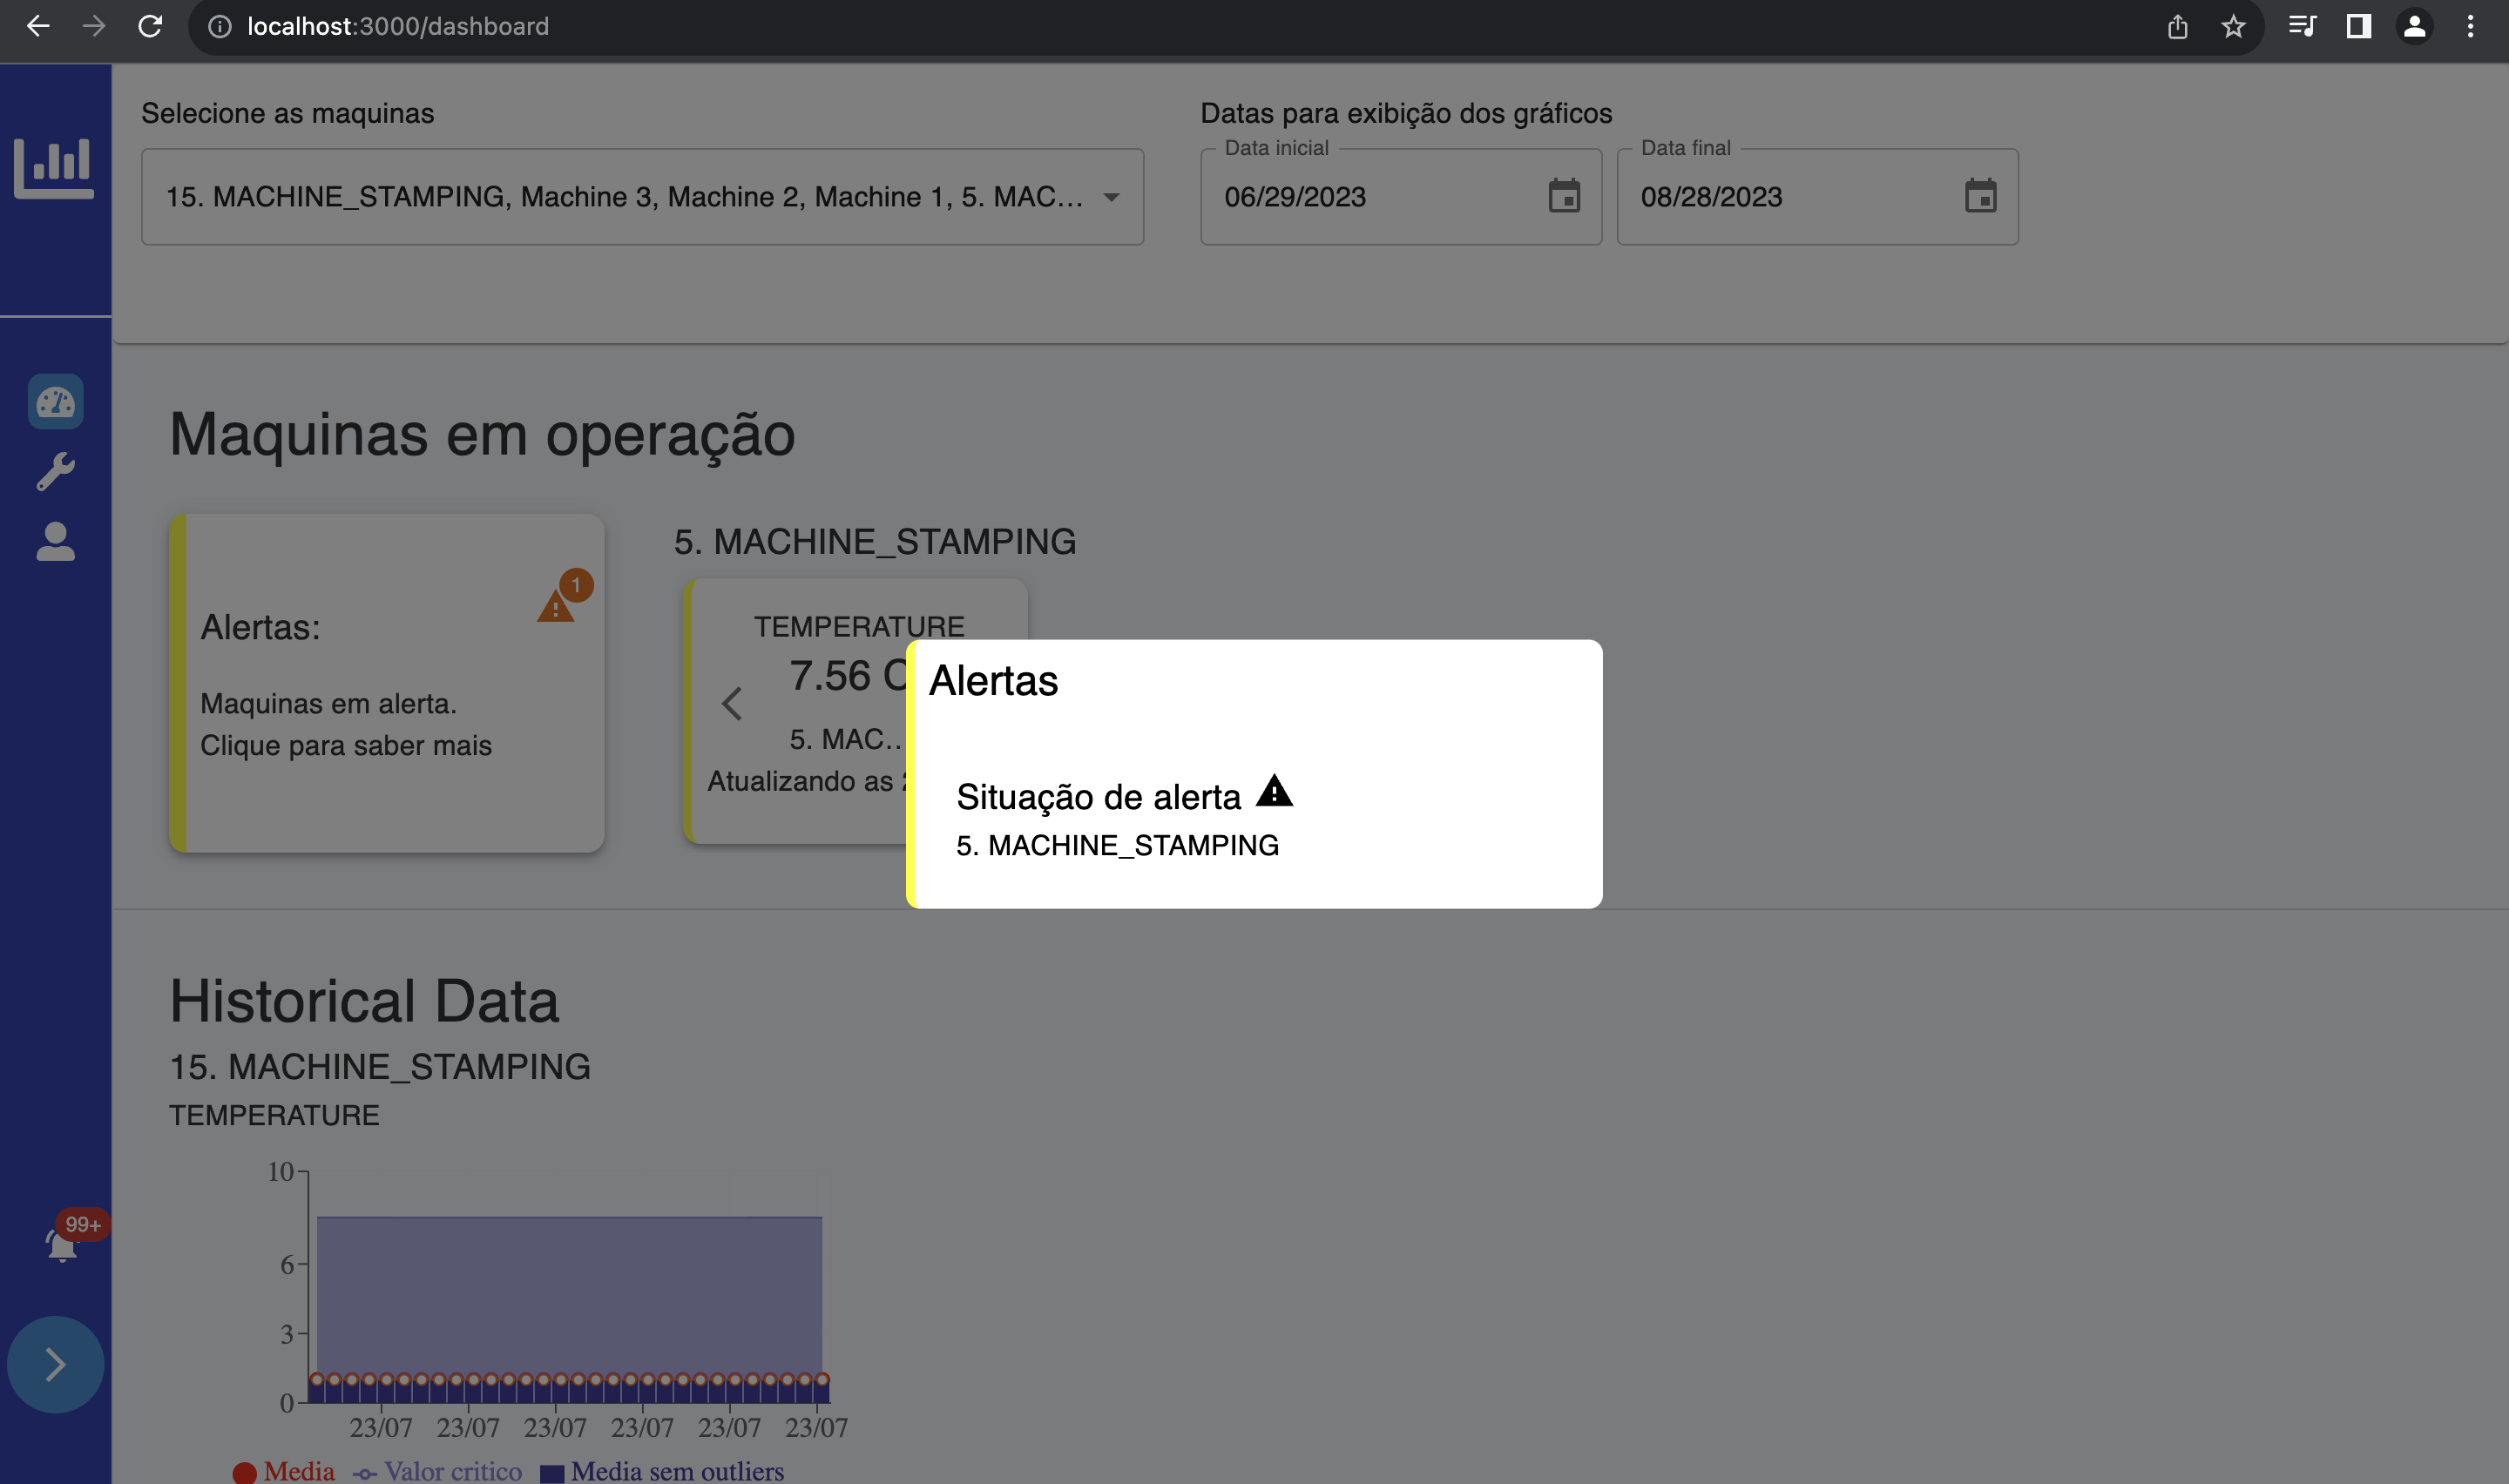
\includegraphics[scale=0.2]{images/geralMachineAlert.png}
	\caption{General Notifications.}
	\label{fig:geralMachineAlert}
\end{figure}

The data receiving module, \ref{sec:Implementation of the data receiving module}, keeps track of the operational state of each machine that is sending information. When a machine exits an alert state, the occurrence is recorded in the database, with the start and end date of the alert state, along with information related to the sensor and the involved machine, as explained in \ref{subsubsec:WebSocketImplement}. Subsequently, a message is sent to the connected users using the \textit{WebSocket} interface, informing them of the machine's malfunction during the period recorded by the system.

Information about alert completion can be accessed by users through notifications in the system interface, as can be seen in figure \ref{fig:notificationDrawer}. By clicking on the notification icon in the dashboard's side menu, the user can view these notifications.

\begin{figure}[htbp]
	\centering
	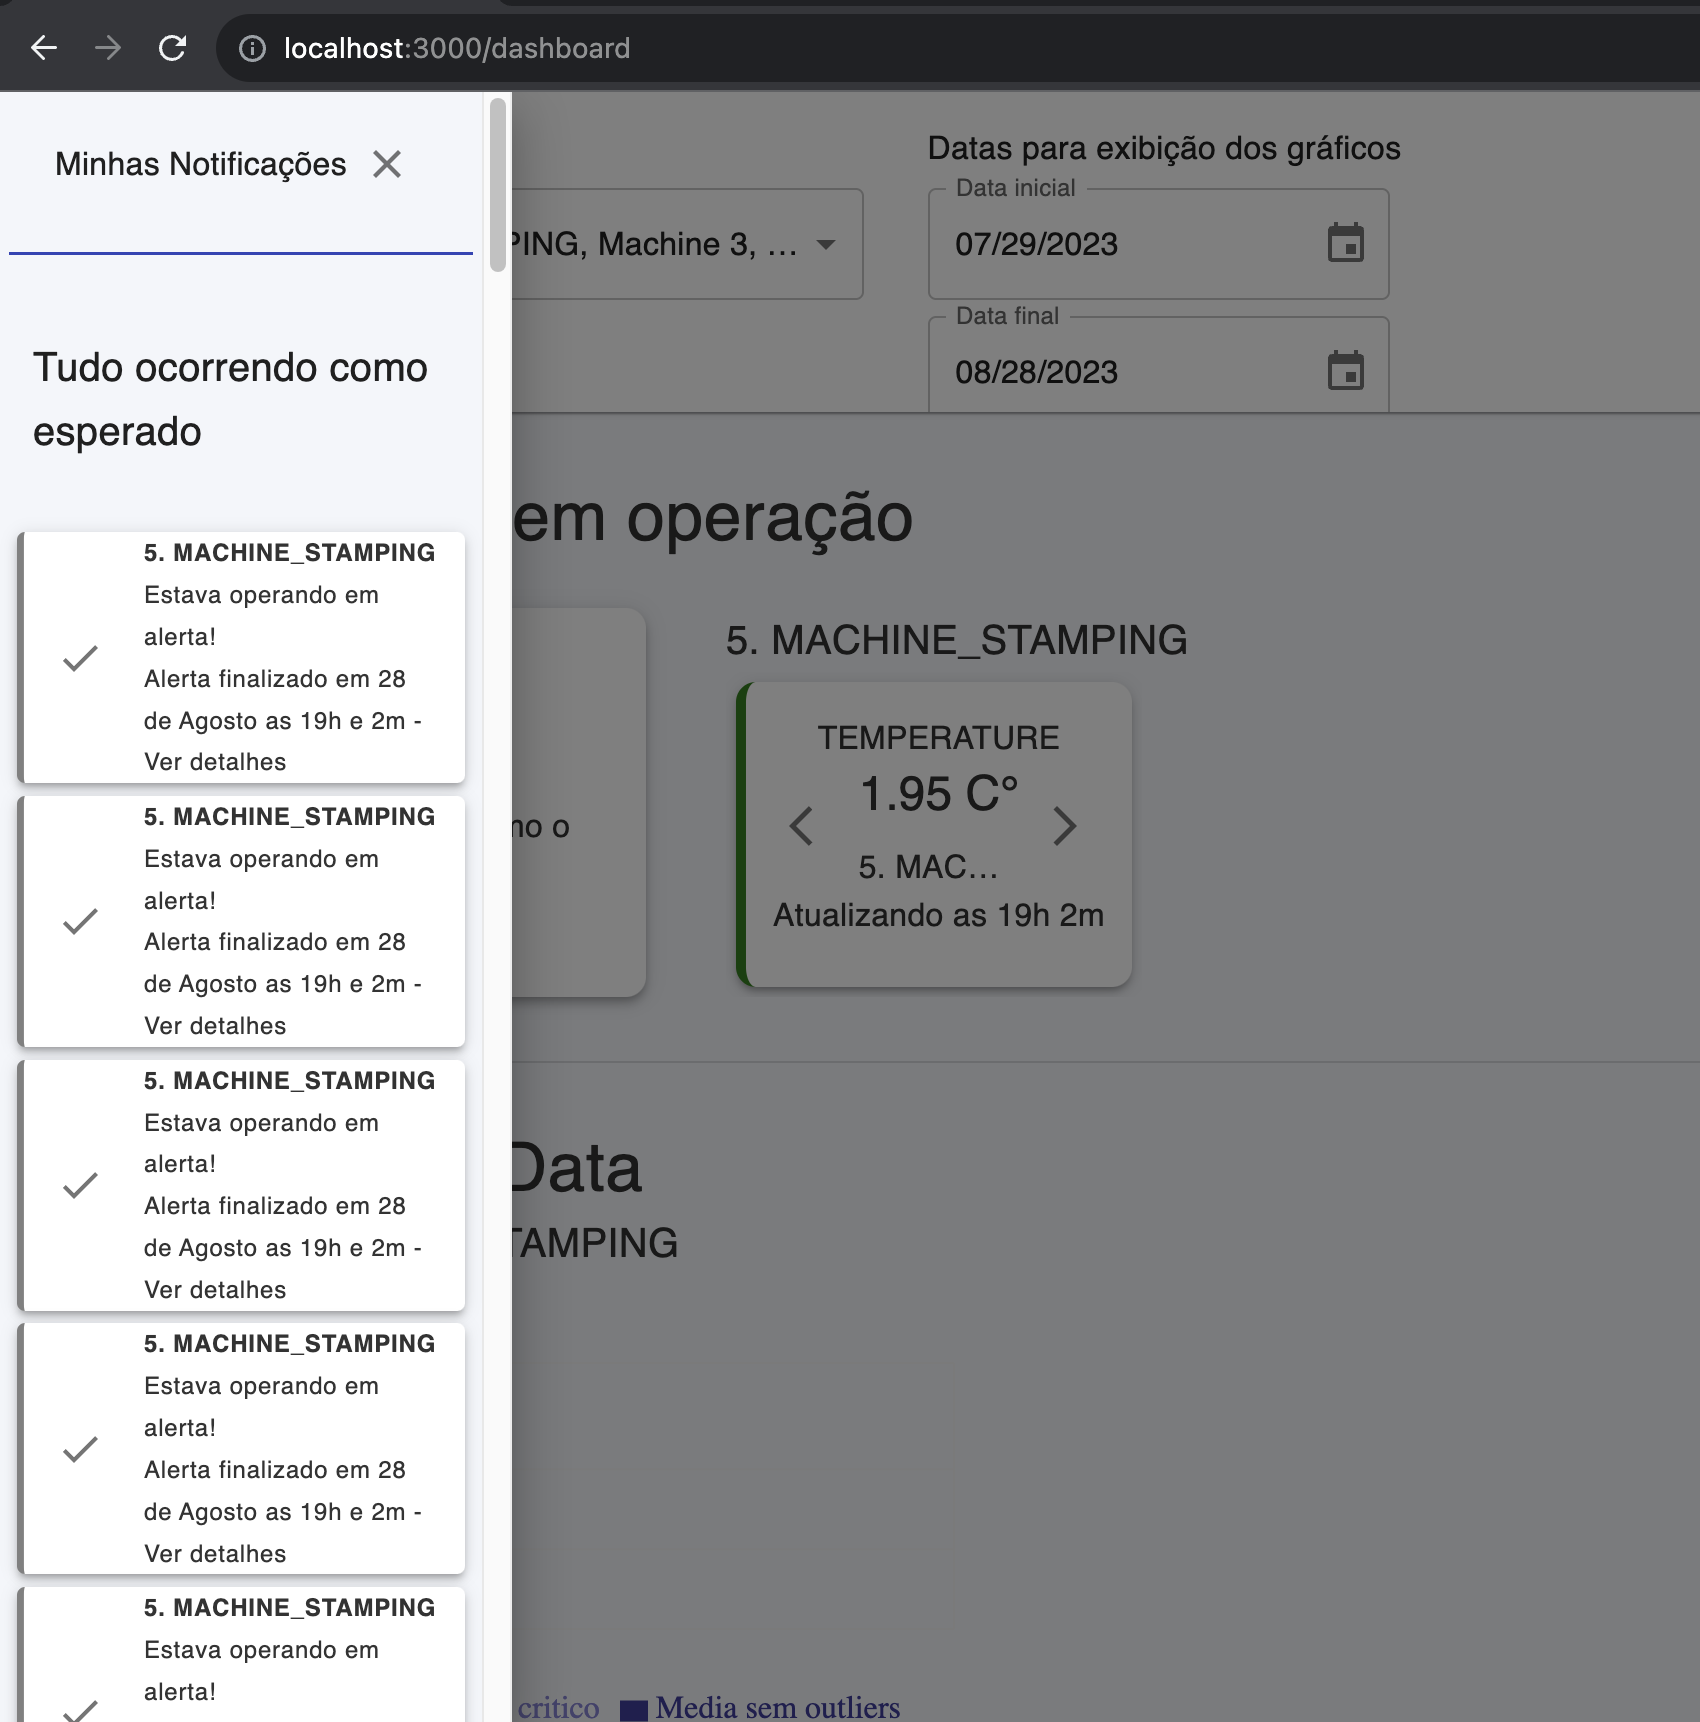
\includegraphics[width=0.6\textwidth]{images/notification.png}
	\caption{Notification drawer.}
	\label{fig:notificationDrawer}
\end{figure}


Therefore, when starting a session in the system, previous notifications are loaded for the user. In addition, any new notification generated during the user's session is transmitted in real time through a WebSocket connection established between the frontend and the backend, as explained in \ref{subsubsec:WebSocketImplement}.


\section[Statistical Analysis of Historical Data]{Statistical Analysis of Historical Data}\label{sec:histicalGraphs}

The data processing module is responsible for the statistical analysis of historical data. Following the system's standard parameter, every day at midnight, the raw unprocessed data is read and analyzed. The result of the analysis is then stored in the database for future queries, as explained in \ref{sec:ImplModuloProcessamento}.

The possibility to access these analytical data is provided by the \gls{API}, specifically by the "IOT Analytics" module. The request to obtain this information must be authenticated, as described in section \ref{subsec:modules}.

The visual representation of these analyses is carried out through graphs that aggregate four main metrics resulting from the processing. Thus, the graph displays:

\begin{itemize}
    \item \textit{Ideal Value}: Represented in an area chart, it serves as an ideal operating parameter to provide a perspective relative to the other data.
    \item \textit{75th Percentile}: Displayed in a line chart, this metric offers a view on the distribution of values during the aggregation period and its evolution over time.
    \item \textit{Aggregation Average}: Represented in a scatter chart, this metric provides the average value of the aggregated data.
    \item \textit{Average with Outlier Removal}: Illustrated in a bar chart, this metric is calculated after the removal of outlier values, as determined by the boxplot construction method.
\end{itemize}

Therefore, image \ref{fig:graphData} shows how these information are displayed within the dashboard.

\begin{figure}[htbp]
	\centering
	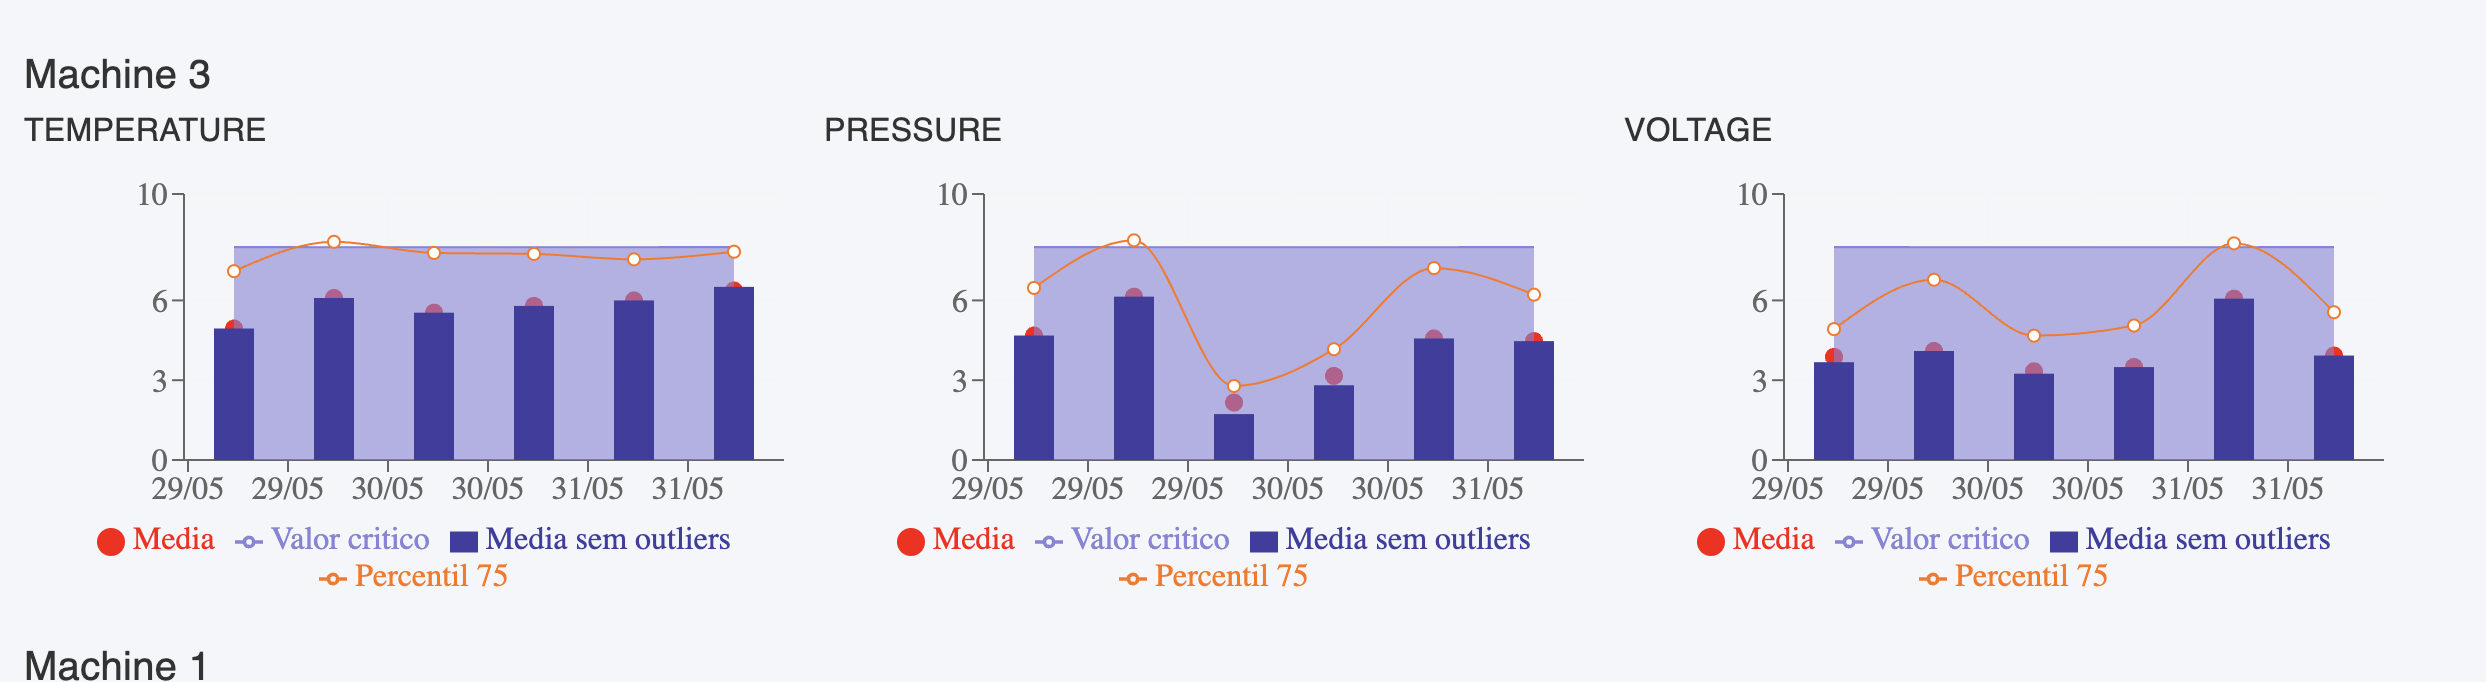
\includegraphics[width=0.7\textwidth]{images/graphData.png}
	\caption{Graph example.}
	\label{fig:graphData}
\end{figure}


The visualization of these graphs can be filtered by date, allowing the selection of the start date and the end date for the data to be displayed. When these fields are changed and the "apply filter" button is clicked, a new request is sent and the data is loaded according to the specified period. By default, when the page is first loaded, the system sends a request seeking data from the last 30 days, and it is up to the user to use the filter to view a different period. The date filter can be seen in figure \ref{fig:loadDataByDate}.

\begin{figure}[htbp]
	\centering
	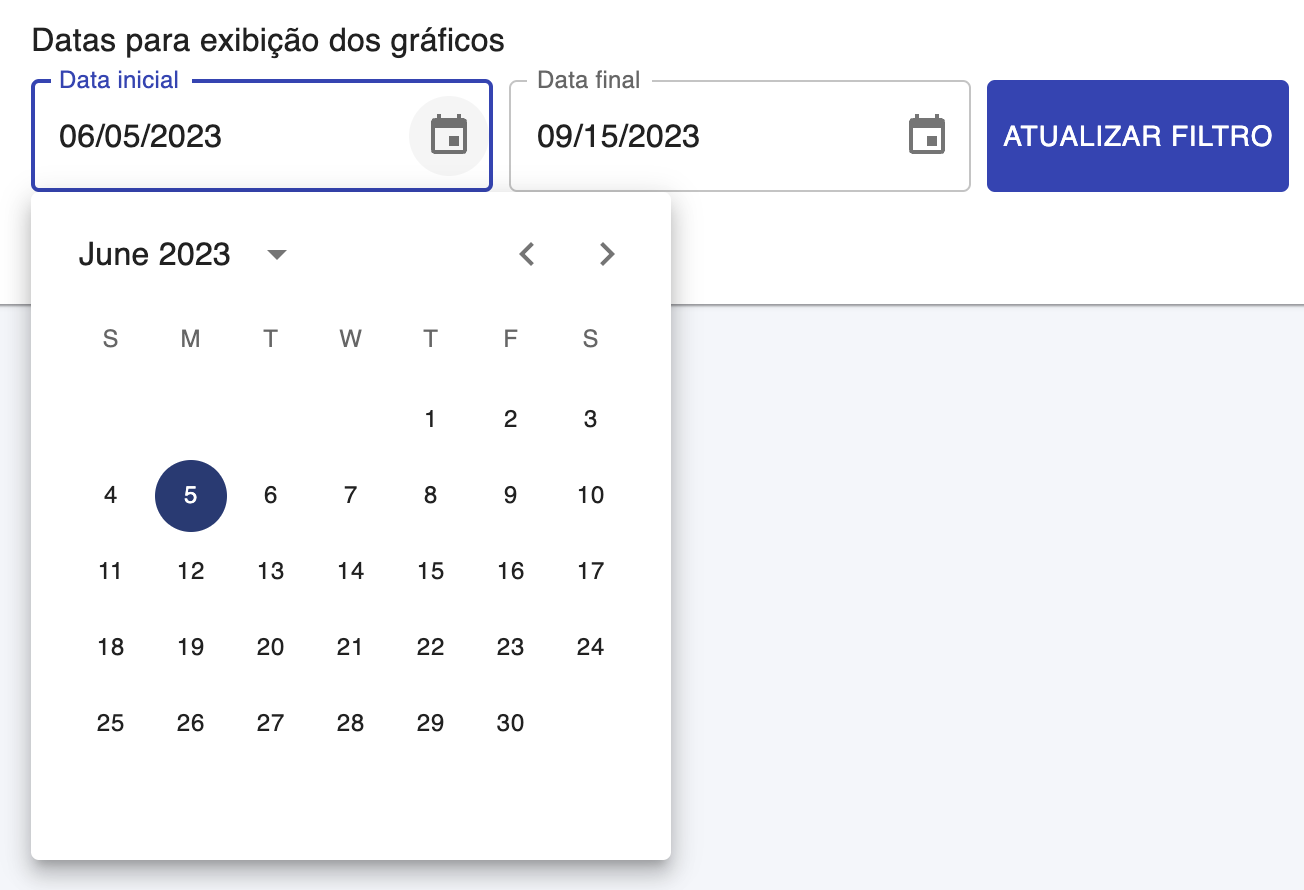
\includegraphics[scale=0.4]{images/datetimeFilter.png}
	\caption{Date filter.}
	\label{fig:loadDataByDate}
\end{figure}

\section[Display of data related to machine downtime]{Display of data related to machine downtime}\label{sec:downtime}

This feature is dedicated to the display of data related to machine downtime, previously stored in the database. The functionality aims to demonstrate how this data would be presented if it were received by the system in a manner similar to sensor data. The source of the data for the preparation of these graphs comes from three spreadsheets received at the beginning of the project development, where the information was saved in the database. This data is accessed by the frontend through the \texttt{downtime\_analytics} module of the \gls{API}.

The graphs generated to represent these data are presented in the form of column charts. Each chart displays a title corresponding to the spreadsheet from which the data were extracted. The chart legend indicates the percentage that each specific stop represents in relation to the total stops.

Column charts provide an effective way to compare the different machine stops, as can be seen in figure \ref{fig:downtime}. This visualization offers a means to analyze operational efficiency, identify possible areas for improvement, and track the outcome of actions taken in relation to machine downtime and predictive maintenance.

\begin{figure}[htbp]
	\centering
	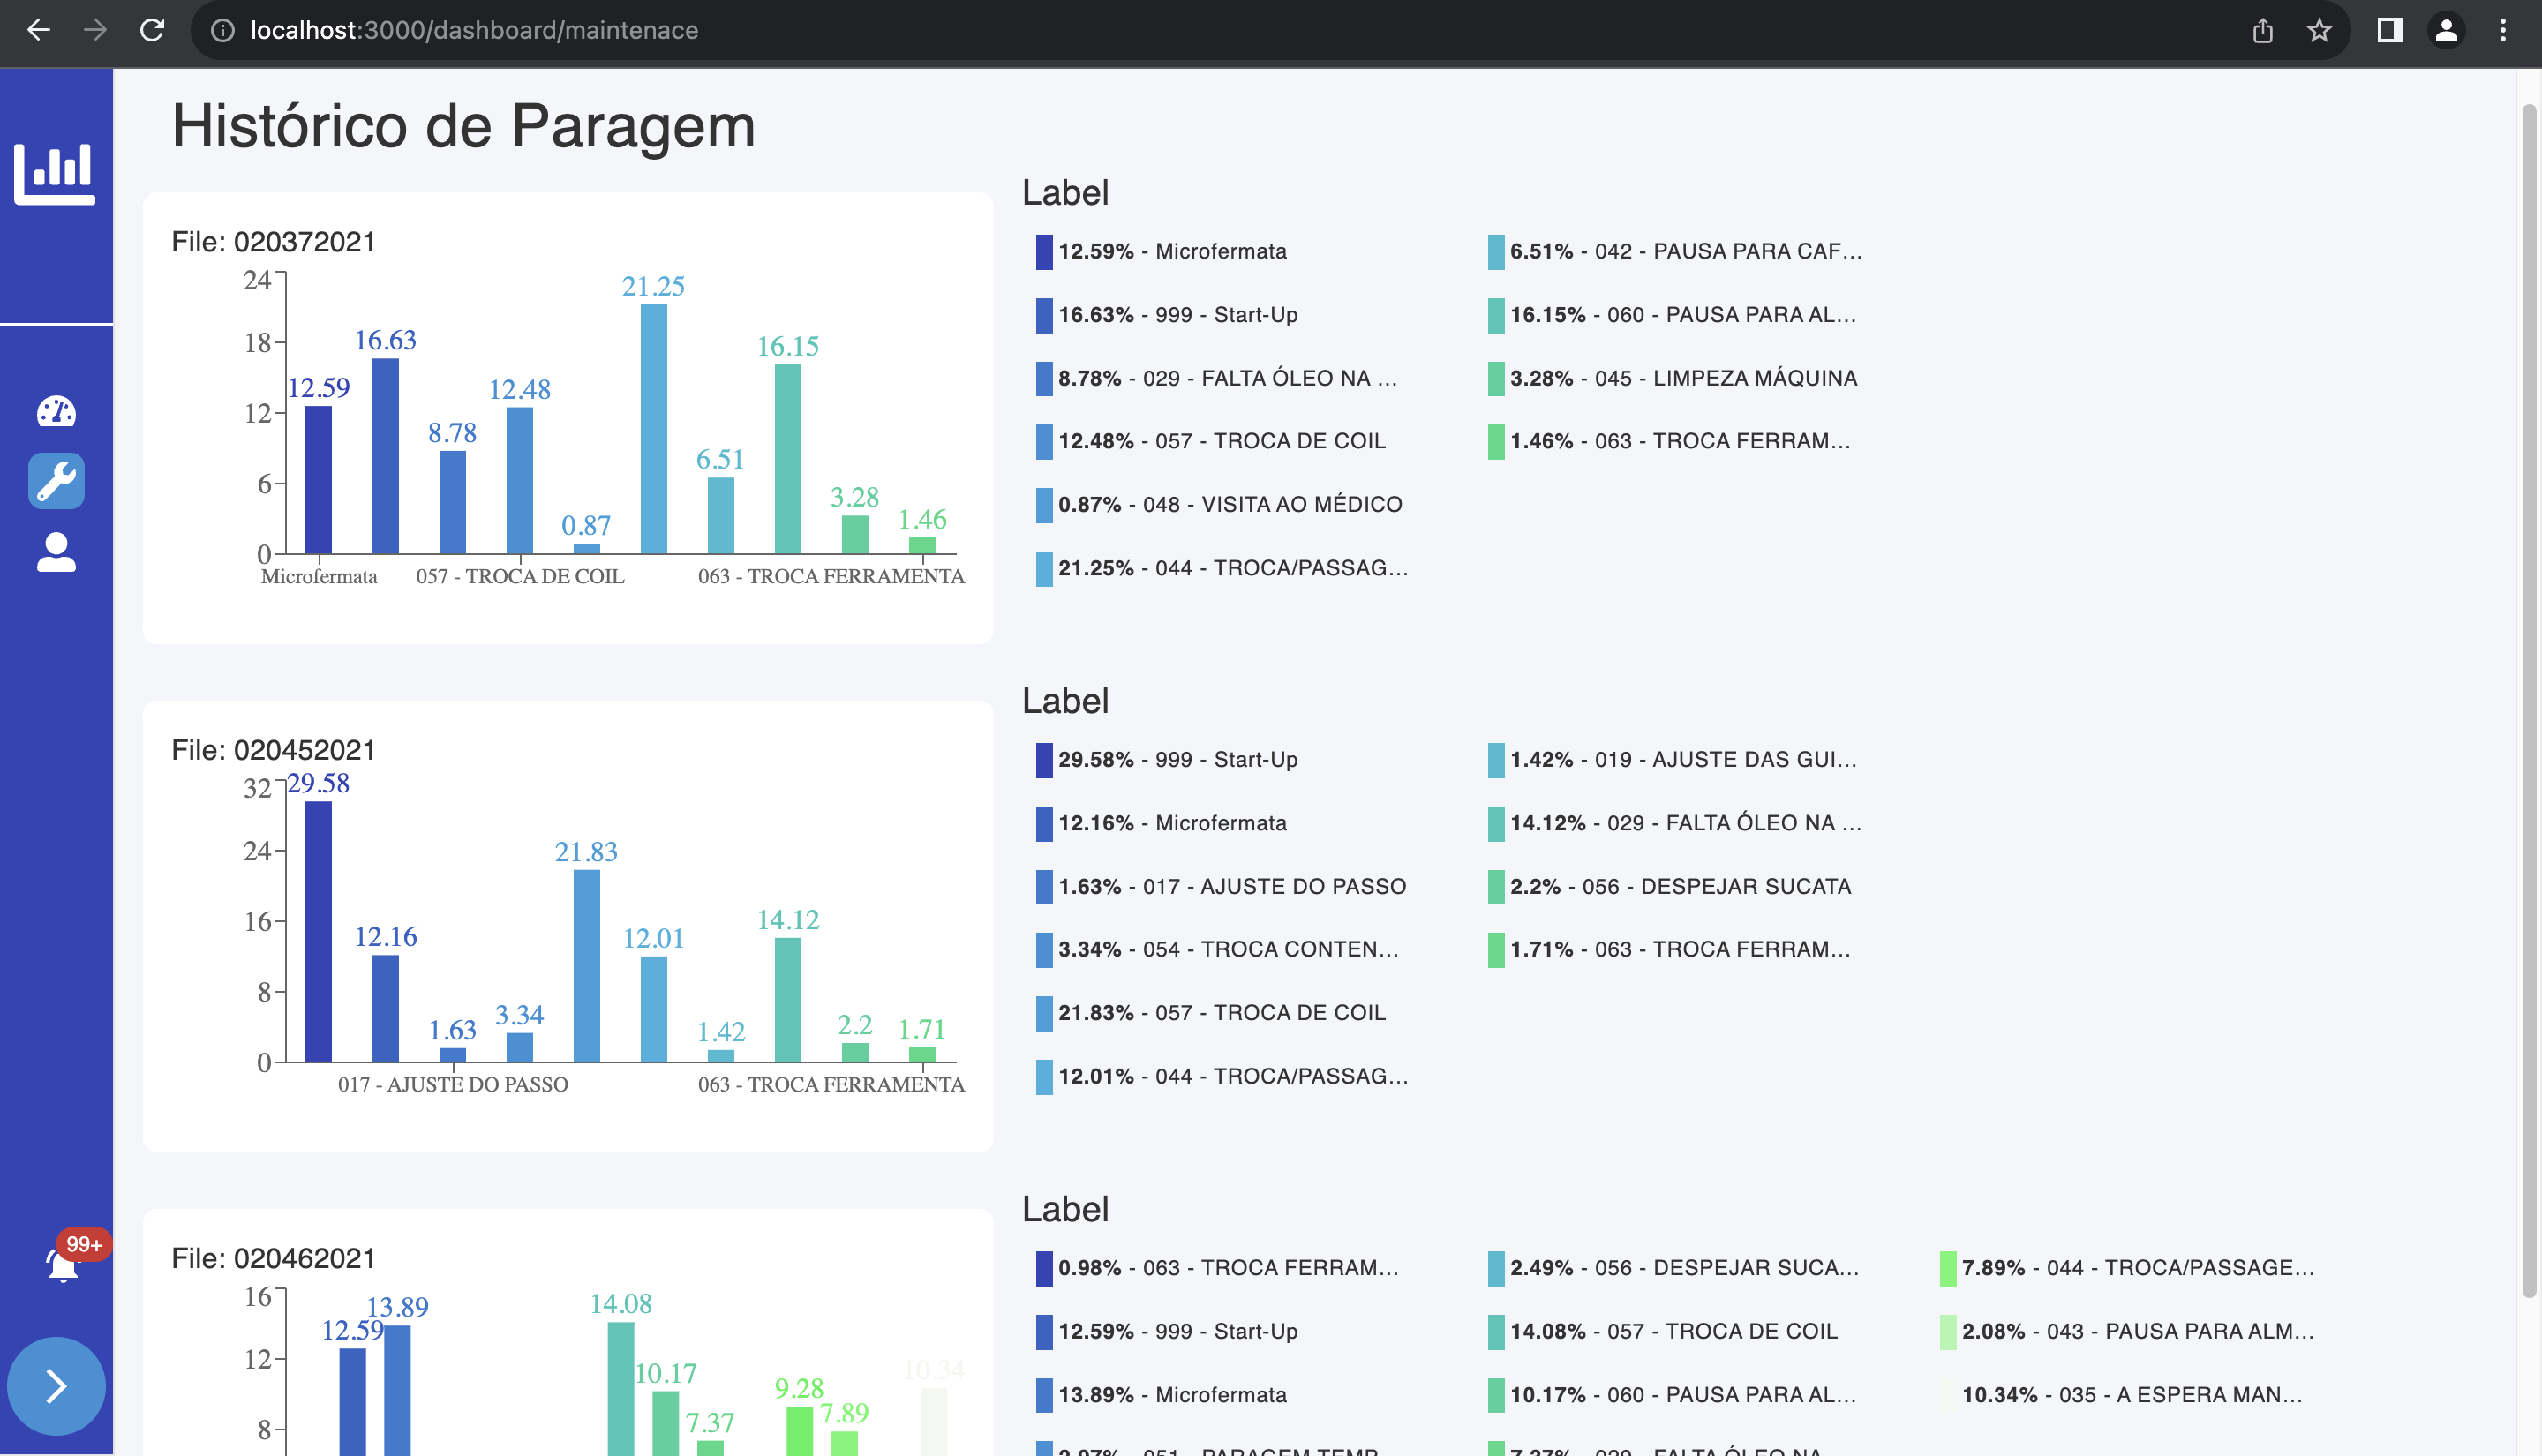
\includegraphics[width=0.75\textwidth]{images/downtime.png}
	\caption{Downtime graph.}
	\label{fig:downtime}
\end{figure}

\section[User Profile]{User Profile}\label{sec:profile}

The user profile functionality was developed with the aim of providing users with access to their personal data stored in the system. In addition to viewing this information, this screen also allows for modifications, including password changes, email, and other personal data such as name, surname, and description.

To read and modify the displayed data, the \textit{User} module of the \gls{API} is used. This module provides endpoints that allow access and modification of the stored data, ensuring that the information is updated according to the user's interactions, as can be seen in figure \ref{fig:profilePage}.

An additional feature provided by this screen is the logout option. By selecting this option, all client-side stored information is erased, thus ensuring the user's secure exit from the system.

\begin{figure}[htbp]
	\centering
	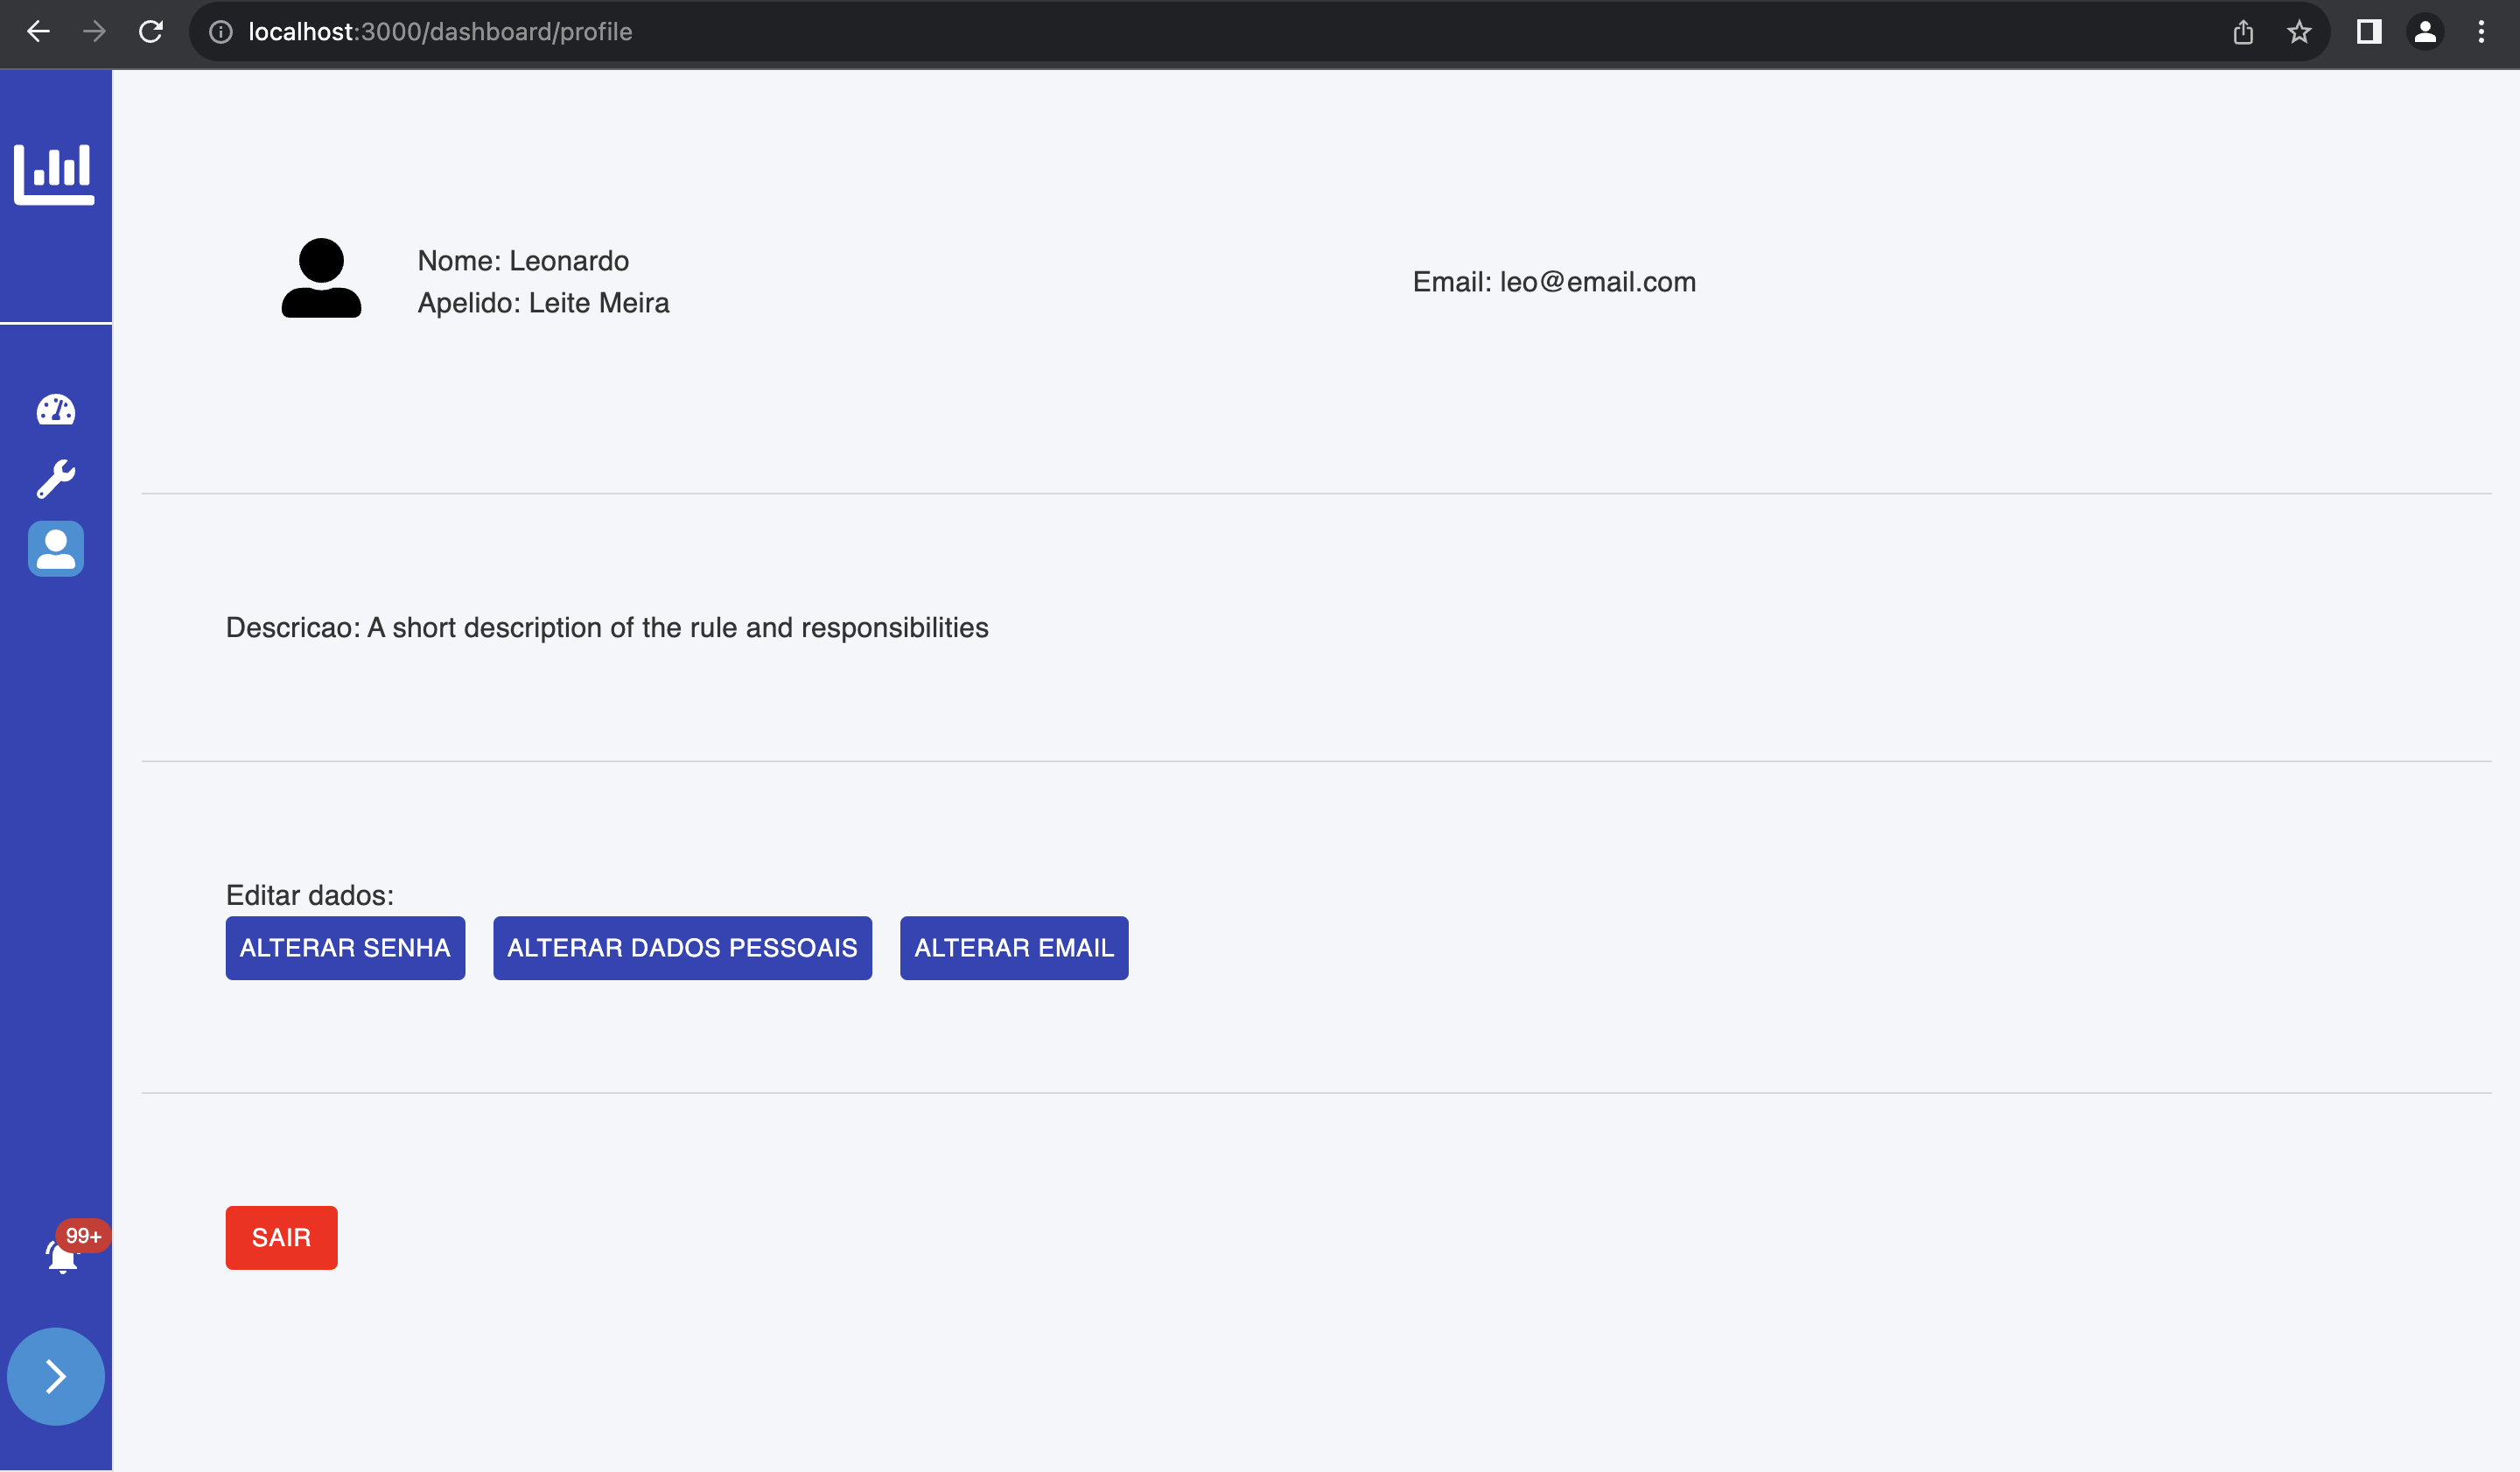
\includegraphics[width=0.8\textwidth]{images/profile.png}
	\caption{Profile page.}
	\label{fig:profilePage}
\end{figure}